\documentclass[notes=show]{beamer}
\usepackage{mathpazo}
\usepackage{hyperref}
\usepackage{multimedia}
\usepackage{tcolorbox}
\usepackage{tikz}
\usetikzlibrary{shadows}
\usetheme{metropolis}
\usecolortheme{default}
\setbeamertemplate{itemize item}{%
    
\begin{tikzpicture}
        \shade[ball color=black!100!yellow, preaction={fill=black,
opacity=.00,transform canvas={xshift=1mm,yshift=-1mm, yscale=0.5}}] (0,0) circle (0.6ex);
    \end{tikzpicture}
}
\setbeamertemplate{itemize subitem}{%
    
\begin{tikzpicture}
        \shade[ball color=black!100!white, preaction={fill=black,
        opacity=.00,transform canvas={xshift=1mm,yshift=-1mm, yscale=0.5}}] (0,0) circle (0.6ex);
    \end{tikzpicture}
}
\setbeamercolor{frametitle}{bg=white}
\setbeamercolor{frametitle}{fg=black}
\setbeamercolor{background canvas}{bg=white}
\setbeamercolor{block body}{bg=mDarkTeal!30}
\setbeamercolor{block title}{bg=mDarkTeal,fg=black!2}
\setbeamertemplate{navigation symbols}{}
\setbeamertemplate{footline}[page number]
\newenvironment{stepenumerate}{\begin{enumerate}[<+->]}{\end{enumerate}}
\newenvironment{stepitemize}{\begin{itemize}[<+->]}{\end{itemize} }
\newenvironment{stepenumeratewithalert}{\begin{enumerate}[<+-| alert@+>]}{\end{enumerate}}
\newenvironment{stepitemizewithalert}{\begin{itemize}[<+-| alert@+>]}{\end{itemize} }

\begin{document}

\title{Artificial Intelligence, Automation, and Work}
\subtitle{}
\date{Daron Acemoglu \& Pascual Restrepo \bigskip \\
\textit{The Economics of Artificial Intelligence}, June 2019 \\
NBER Conference Volume, Chapter 8}
\author{}
\maketitle

\begin{frame}{Table of Contents}
\begin{itemize}
\item[\textcolor{gray}{8.1}] \textcolor{gray}{Introduction} \medskip
\item[\textcolor{gray}{8.2}] \textcolor{gray}{Automation, Work , and Wages: An Overview} \medskip
\item[\textcolor{black}{8.3}] \textcolor{black}{A Model of Automation, Tasks, and the Demand for Labor} \medskip
\item[\textcolor{black}{8.4}] \textcolor{black}{Technology and Labor Demand} \medskip
\item[\textcolor{black}{8.5}] \textcolor{black}{Flies in the Ointment} \medskip
\item[\textcolor{black}{8.6}] \textcolor{black}{Conclusions}
\end{itemize}
\end{frame}

\section{8.3. A Model of Automation, Tasks, and the Demand for Labor}

\newpage
\begin{center}
\begin{figure}
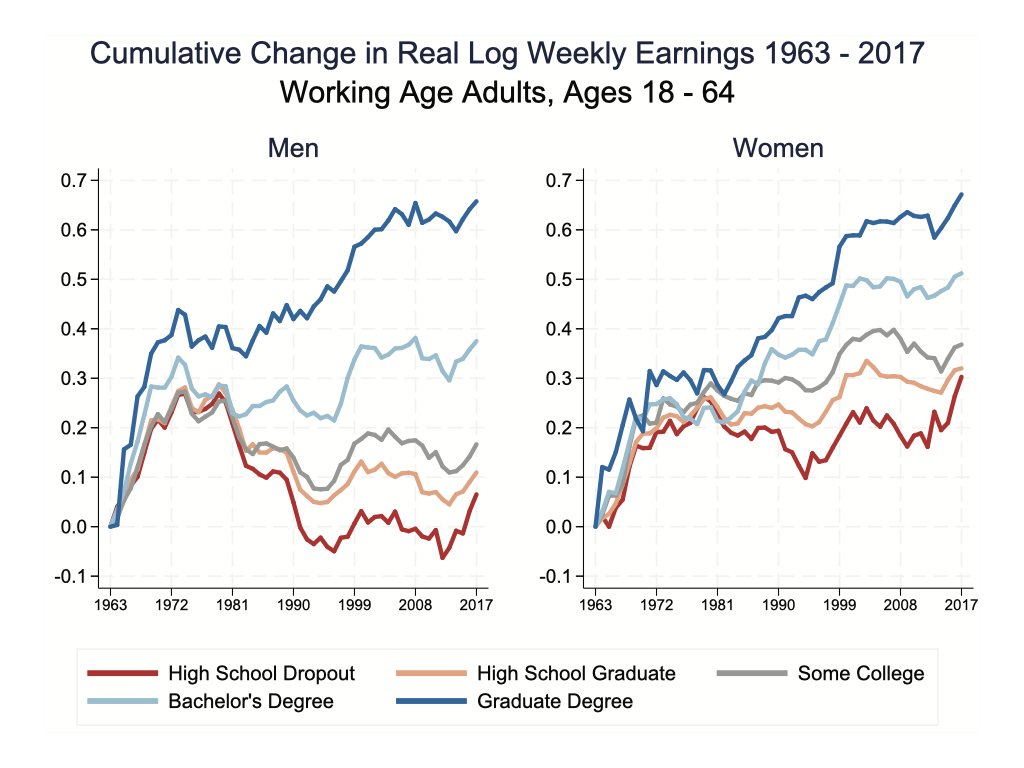
\includegraphics[height=8.5cm,width=\textwidth]{figureM1.png} 
\end{figure}
\end{center}
\newpage

\newpage
\begin{center}
\begin{figure}
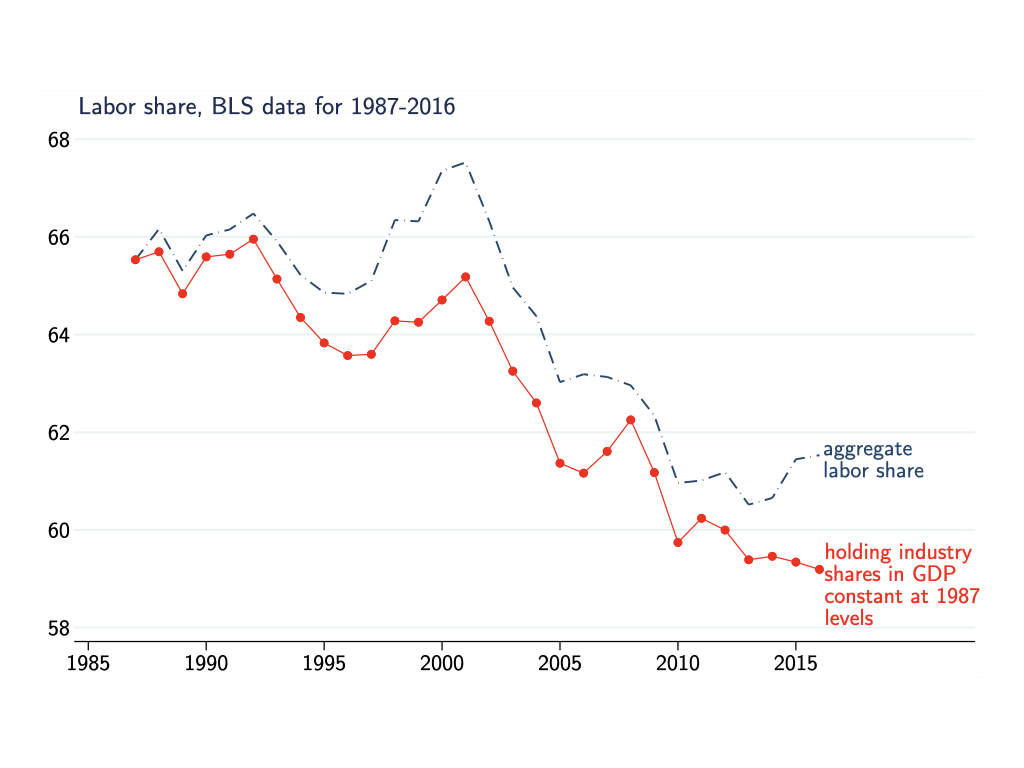
\includegraphics[height=8.5cm,width=\textwidth]{figureM2.png}
\end{figure}
\end{center}
\newpage

\begin{frame}{Motivation (Acemoglu \& Restrepo [18])}
\begin{itemize}
\item \textbf{2-factor CRS production functions assuming factor-augmenting technological change} pose important problems and puzzles. \medskip
\item \textbf{Capital-augmenting} technological change cannot explain declining wages for some workers or the recent fall in the labor share for realistic parameter values. \medskip
\item \textbf{Labor-augmenting} technological change cannot explain declining wages for realistic parameter values. \medskip
\item It could explain the recent fall in the labor share for realistic parameter values, but it is not very convincing conceptually.
\end{itemize}
\end{frame}

\subsection{8.3.1 A task-based framework}

\begin{frame}{8.3 A model of automation, tasks, and the demand for labor}
\begin{itemize}
\item[\textcolor{red}{8.3.1}] \textcolor{red}{A task-based framework} \bigskip
\item[\textcolor{gray}{8.3.2}] \textcolor{gray}{Types of technological change} \bigskip
\item[\textcolor{gray}{8.3.3}] \textcolor{gray}{Equilibrium}
\end{itemize}
\end{frame}

\begin{frame}{Production technology}
\begin{itemize}
\item Static environment with a unique final good, $Y$. \medskip
\item $Y$ is produced with a continuum of tasks on the unit interval $[N-1,N]$ with $N$ an exogenous parameter. \medskip
\item Cobb-Douglas technology mapping tasks into the final good:
\[
Y= \exp \left[ \int_{N-1}^{N} \ln y(z)dz \right] \tag{1}  \label{eq1}
\]
where $y(z)$ is the service or production of task $z$. \medskip
\item The final good is the numeraire, $P \equiv 1$.
\end{itemize}
\end{frame}

\begin{frame}{The frontier of automation possibilities}
\begin{block}{Assumptions}
\begin{itemize}
\item Tasks $z \in [N-1,N]$ are ranked such that they become increasingly more difficult for machines to do. \medskip
\item Assume an exogenous threshold $I$ which is the frontier of automation possibilities. \medskip
\item All tasks $z \leq I$ can (and will) be automated, and all tasks $z > I $ can only be done by labor. \medskip
\item An increase in $I$ willl capture automation. 
\end{itemize}
\end{block}
\end{frame}

\begin{frame}{Supply of labor and capital to tasks}
\begin{itemize}
\item Task $z$ can be produced by labor, $l(z)$ or by capital, $k(z)$, according to \underline{equation (2)} given by:
\[
y(z) = 
\begin{cases}
A^{L} \gamma^{L}(z)l(z) + A^{K} \gamma^{K}(z)k(z) \text{ if } z \in [N-1,I]\\
A^{L} \gamma^{L}(z)l(z) \text{ if } z \in (I,N] 
\end{cases} \label{eq2}
\]
where:
\begin{itemize}
\item $A^{L}, A^{K}$ are factor-augmenting technologies \medskip
\item $ \gamma^{L}(z), \gamma^{K}(z)$ are task productivity schedules \medskip
\item $ l(z), k(z)$ are the number of each factor allocated to task $z$
\end{itemize}
\end{itemize}
\end{frame}

\begin{frame}{Comparative advantage in task production}
\begin{block}{Assumption}
$ \gamma^{L}(z)/\gamma^{K}(z)$ is strictly increasing in $z$.
\end{block}
\begin{itemize}
\item This is an assumption about the \textit{relative} productivity of labor and capital in doing different tasks. \medskip
\item This assumption drives their allocation across tasks based on comparative advantage (as in Roy [51]).\medskip
\item All tasks $z \in [N-1,I]$ will be done by capital and all tasks $z \in (I,N]$ will be done by labor. 
\end{itemize}
\end{frame}

\newpage
\begin{center}
\begin{figure}
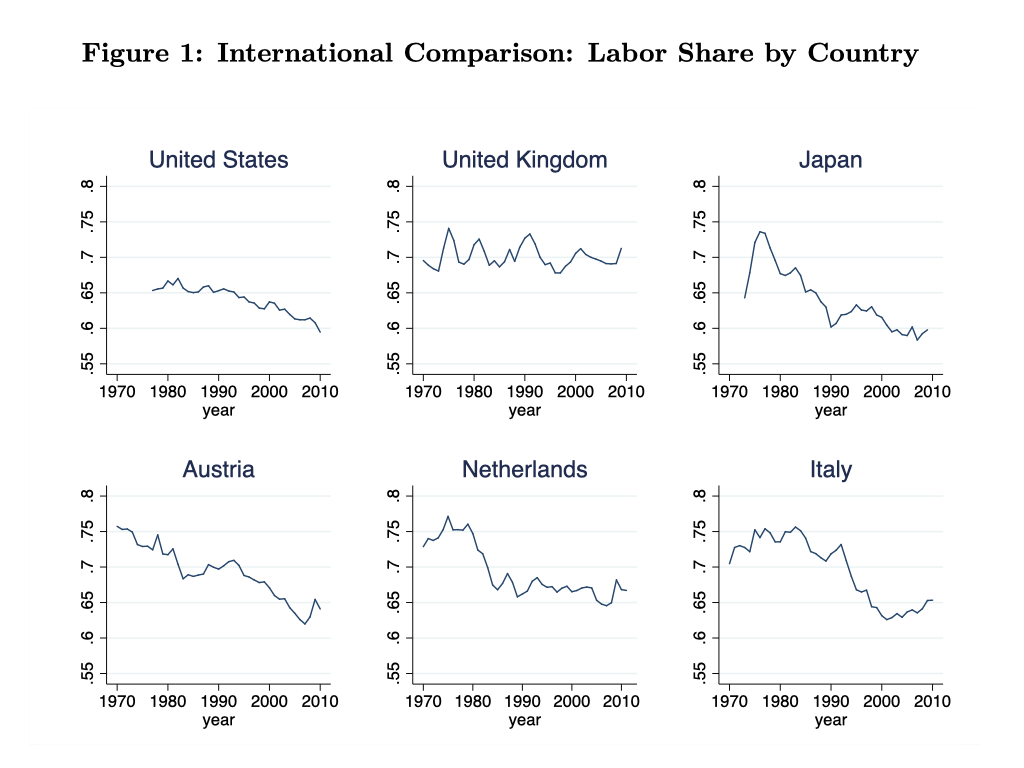
\includegraphics[height=7.5cm,width=\textwidth]{figure1a.png}
\\ Allocation of tasks to factors 
\end{figure} 
\end{center}
\newpage

\begin{frame}{Clearing factor markets}
\begin{itemize}
\item Labor and capital are supplied inelastically by $L$ and $K$ respectively. \medskip
\item Labor markets clearing requires:
\[
\int_{N-1}^{N} l(z)dz = L \text{ and } \int_{N-1}^{N} k(z)dz = K
\]
\item In this environment, we can look at: \medskip
\begin{itemize}
\item Types of technologies and equilibrium (sections 8.3.2-8.3.3) \medskip
\item Technology and labor demand (section 8.4) \medskip
\item Flies in the ointment (section 8.5)
\end{itemize}
\end{itemize}
\end{frame}

\subsection{8.3.2 Types of technological change}

\begin{frame}{8.3 A model of automation, tasks, and the demand for labor}
\begin{itemize}
\item[\textcolor{gray}{8.3.1}] \textcolor{gray}{A task-based framework} \bigskip
\item[\textcolor{red}{8.3.2}] \textcolor{red}{Types of technological change} \bigskip
\item[\textcolor{gray}{8.3.3}] \textcolor{gray}{Equilibrium}
\end{itemize}
\end{frame}

\newpage
\begin{center}
\begin{figure}
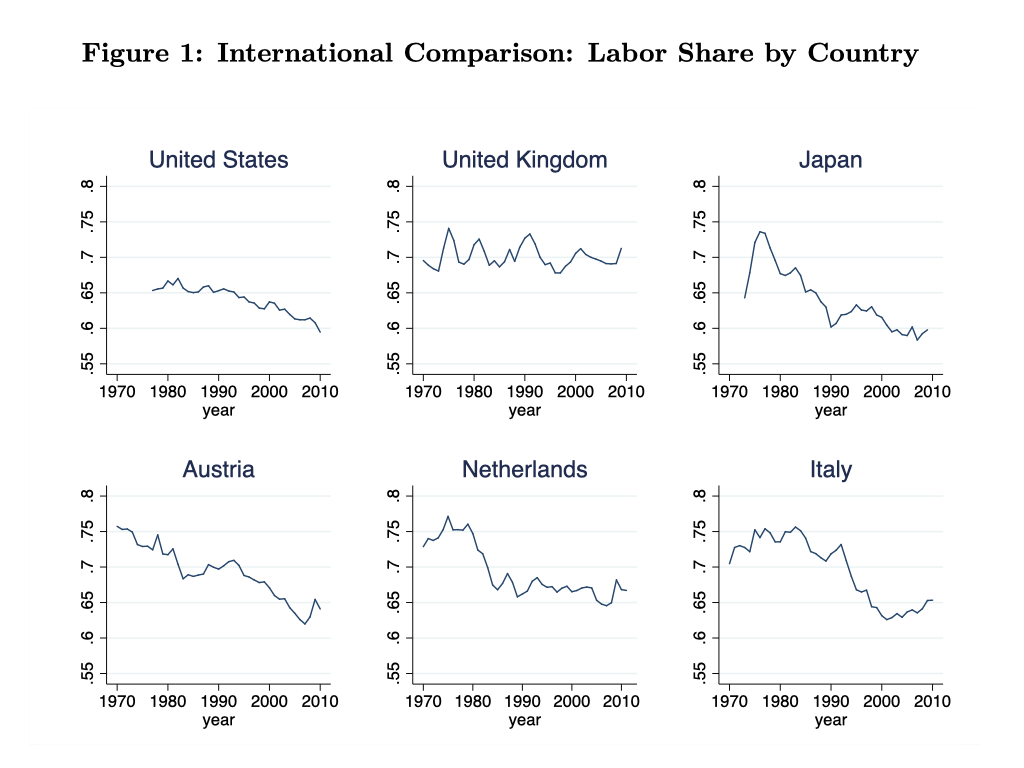
\includegraphics[height=7.5cm,width=\textwidth]{figure1a.png}
\\ Allocation of tasks to factors 
\end{figure} 
\end{center}
\newpage

\begin{frame}{Types of technological change}
\begin{enumerate}
\item \textbf{Labor-augmenting technological change}: \\
$A^{L} \uparrow$ or $\gamma^{L}(z) \uparrow$ for all $z$\medskip
\item \textbf{Automation (at the extensive margin)}: \\
Automation possibility frontier $I \uparrow $ \medskip
\item \textbf{Deepening of automation (at the intensive margin)}: \\
$A^{K} \uparrow$ or $\gamma^{K}(z) \uparrow$ for all $z < I$ \medskip
\item \textbf{Creation of new labor-intensive tasks}: \\
$N \uparrow $ which increases the bounds of the unit interval of tasks ranked by labor's comparative advantage
\end{enumerate}
\end{frame}

\newpage
\begin{center}
\begin{figure}
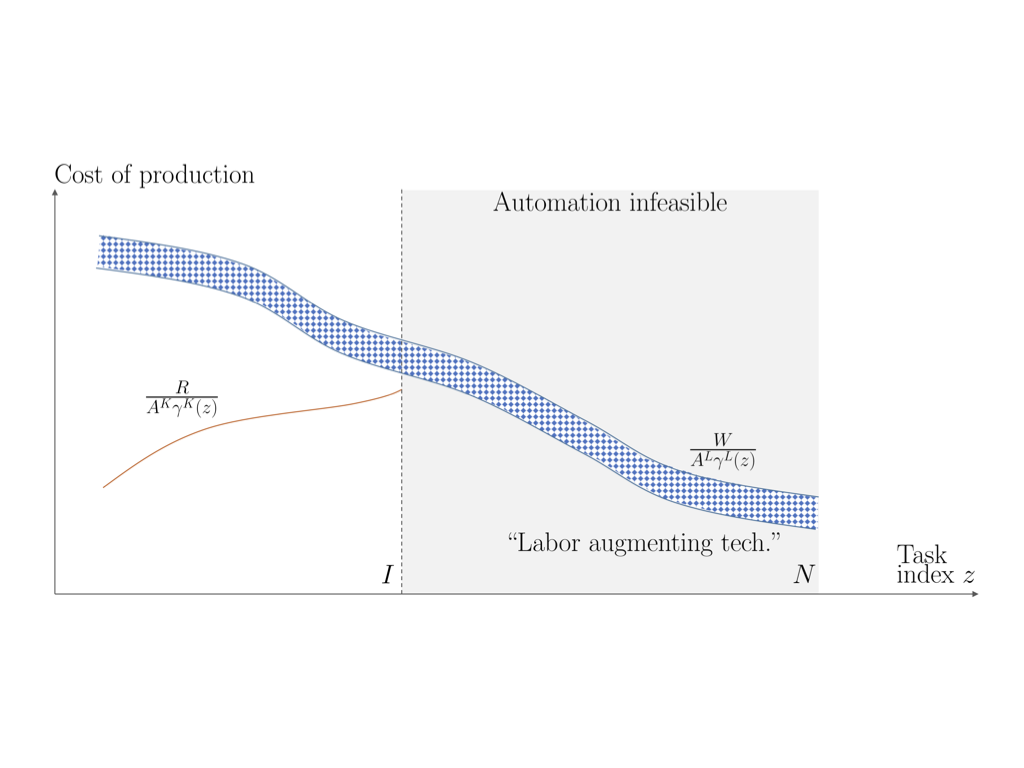
\includegraphics[height=7.5cm,width=\textwidth]{figure1c.png}
\\ 1. \textbf{Labor-augmenting technological change}: \\
$A^{L} \uparrow$ or $\gamma^{L}(z) \uparrow$ for all $z$
\end{figure} 
\end{center}
\newpage

\newpage
\begin{center}
\begin{figure}
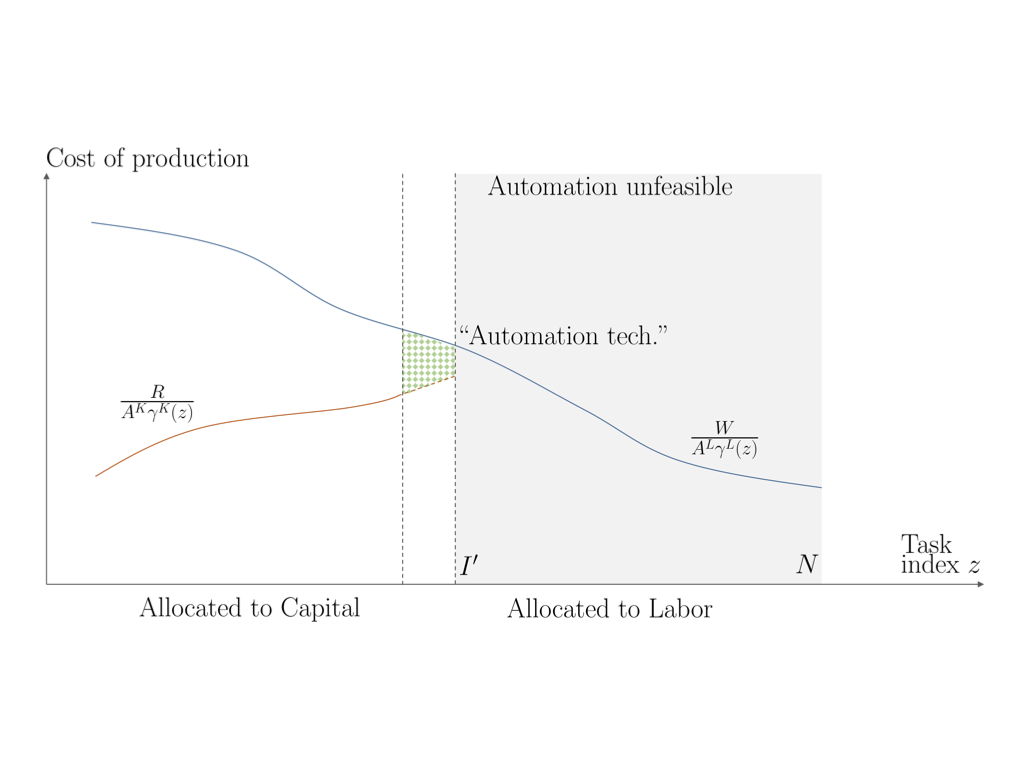
\includegraphics[height=7.5cm,width=\textwidth]{figure1d.png}
\\ 2. \textbf{Automation (at the extensive margin)}: \\
Automation possibility frontier $I \uparrow $
\end{figure} 
\end{center}
\newpage

\newpage
\begin{center}
\begin{figure}
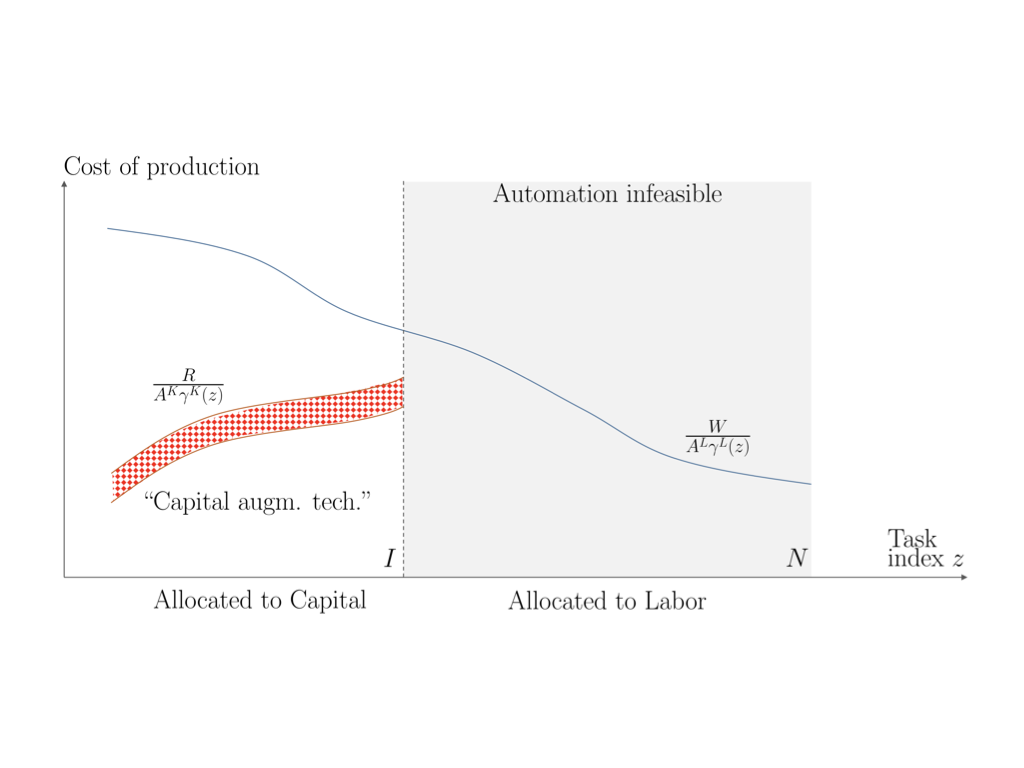
\includegraphics[height=7.5cm,width=\textwidth]{figure1b.png}
\\ 3. \textbf{Deepening of automation (at the intensive margin)}: \\
$A^{K} \uparrow$ or $\gamma^{K}(z) \uparrow$ for all $z < I$
\end{figure} 
\end{center}
\newpage

\newpage
\begin{center}
\begin{figure}
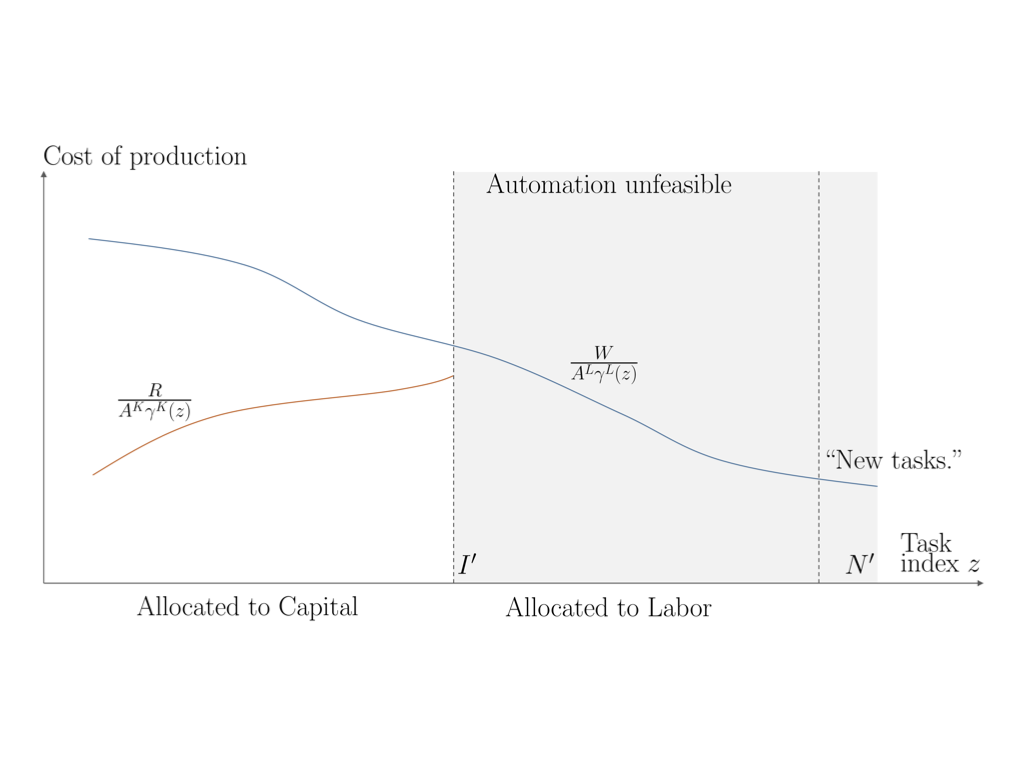
\includegraphics[height=7cm,width=\textwidth]{figure1e.png}
\\ 4. \textbf{Creation of new labor-intensive tasks}: \\
$N \uparrow $ which increases the bounds of the unit interval of tasks ranked by labor's comparative advantage
\end{figure} 
\end{center}
\newpage

\subsection{8.3.3 Equilibrium}

\begin{frame}{8.3 A model of automation, tasks, and the demand for labor}
\begin{itemize}
\item[\textcolor{gray}{8.3.1}] \textcolor{gray}{A task-based framework} \bigskip
\item[\textcolor{gray}{8.3.2}] \textcolor{gray}{Types of technological change} \bigskip
\item[\textcolor{red}{8.3.3}] \textcolor{red}{Equilibrium}
\end{itemize}
\end{frame}

\newpage
\begin{center}
\begin{figure}
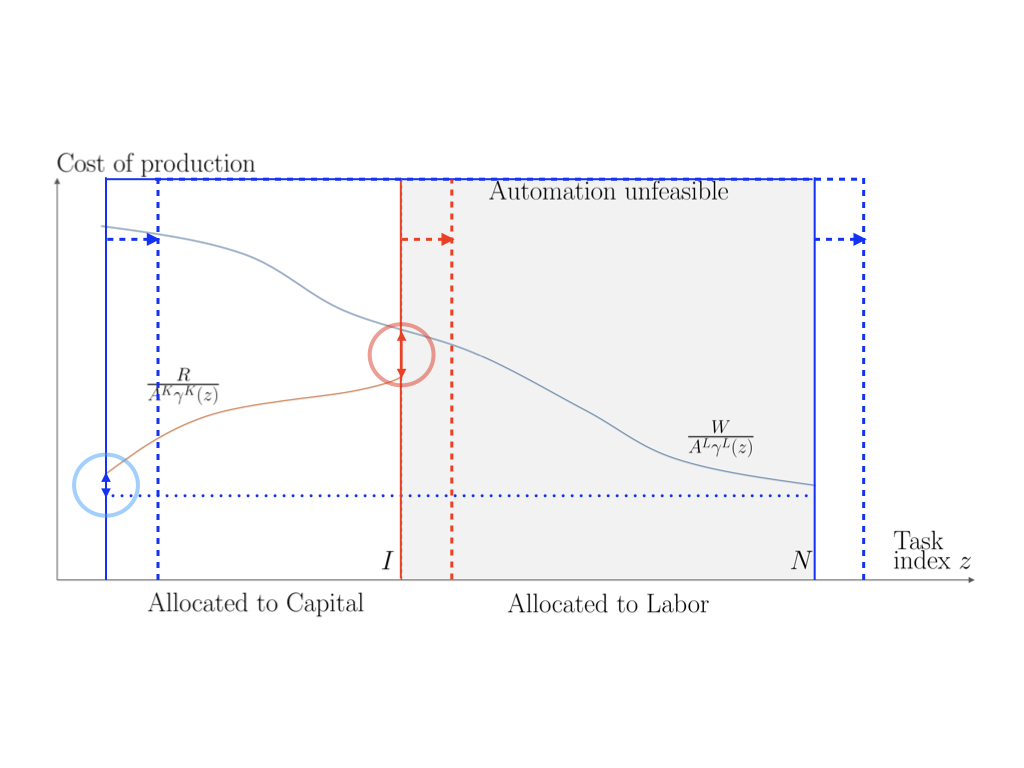
\includegraphics[height=7.5cm,width=\textwidth]{figure1f.png}
\\ Efficiencies at marginal tasks: equilibrium assumptions
\end{figure} 
\end{center}
\newpage

\begin{frame}{Efficiencies at marginal tasks: equilibrium assumptions}
\begin{itemize}
\item Denote the equilibrium wage rate by $W$ and rental rate by $R$. \medskip
\item Further assume that in any equilibrium:
\[
\color{red} \frac{A^{L}\gamma^{L}(I)}{A^{K}\gamma^{K}(I)} < \color{black} \frac{W}{R} \color{blue} < \frac{A^{L}\gamma^{L}(N)}{A^{K}\gamma^{K}(N-1)} \color{black} \tag{A1} \label{eqA1}
\]
\item First inequality implies that all tasks $z \in [N-1,I]$ will be produced by capital and that an increase in $I$ increases $Y$. \medskip
\item Second inequality implies that an increase in $N$ increases $Y$. \medskip
\item We return to these equilibrium assumptions below. 
\end{itemize}
\end{frame}

\begin{frame}{Task demands}
\begin{itemize}
\item Cobb-Douglas mapping a unit interval of tasks:
\[
Y= \exp \left[ \int_{N-1}^{N} \ln y(z)dz \right] \text{ implies that } \forall z: p(z)y(z) = Y
\] 
\item Demand for task $z$ is therefore given by:
\[
y(z) = Y / p(z)
\] 
with the price of task $z$, $p(z)$, given by:
\[
p(z) = 
\begin{cases}
\frac{R}{A^{K} \gamma^{K}(z)} \text{ if } z \in [N-1,I] \\
\frac{W}{A^{L} \gamma^{L}(z)} \text{ if } z \in (I,N] 
\end{cases}
\]
\end{itemize}
\end{frame}

\begin{frame}{Factor demands in tasks}
\begin{itemize}
\item Using that $y(z) = A^{K} \gamma^{K}(z)k(z)$ for $z \in [N-1,I]$:
\[
k(z)=
\begin{cases}
\frac{Y}{R} \text{ if } z \in [N-1,I] \\
0 \text{ if } z \in (I,N]
\end{cases}
\]
which gives demand for capital in each task $z$. \medskip
\item Using that $y(z) = A^{L} \gamma^{L}(z)l(z)$ for $z \in (I,N]$:
\[
l(z)=
\begin{cases}
0 \text{ if } z \in [N-1,I] \\
\frac{Y}{W} \text{ if } z \in (I,N]
\end{cases}
\]
which gives labor demand in each task $z$.
\end{itemize}
\end{frame}

\begin{frame}{Aggregate factor demands}
\begin{itemize}
\item The market clearing condition for capital is:
\[
K = \int_{N-1}^{N} k(z)dz = \frac{Y}{R} \int_{N-1}^{I} dz = \frac{Y}{R}[I-N+1] 
\]
\item The market clearing condition for labor is:
\[
L = \int_{N-1}^{N} l(z)dz = \frac{Y}{W}  \int_{I}^{N} dz = \frac{Y}{W}[N-I]
\]
\item Solving and re-arranging terms gives:
\[
R = \frac{Y}{K}[I-N+1] \text{ and }  W = \frac{Y}{L}[N-I]
\]
\end{itemize}
\end{frame}

\begin{frame}{Equilibrium rental rate, wage and factor shares}
\begin{itemize}
\item The equilibrium rental rate and wage are given by:
\begin{tcolorbox}
\[
R = \frac{Y}{K}[I-N+1] \text{ and }  W = \frac{Y}{L}[N-I] \tag{5} \label{eq5}
\]
\end{tcolorbox}
\item Factor shares in equilibrium are given by:
\begin{tcolorbox}
\[
s_{K} = \frac{RK}{Y} = I-N+1 \text{ and }  s_{L} = \frac{WL}{Y} = N-I  \tag{6} \label{eq6}
\]
\end{tcolorbox}
\item \textbf{Sneak preview}: Automation and new tasks (i.e. an increase in $I$ and $N$) affect the labor share (whereas factor-augmenting technological change does not affect the labor share).
\end{itemize}
\end{frame}

\begin{frame}{Aggregate output in equilibrium}
\begin{itemize}
\item Profit maximization and the final good as the numeraire imply:
\[
P = MC = \exp \left[ \int_{N-1}^{N} \ln(p(z))dz \right] \equiv 1
\]
\item Using expressions for $p(z)$ gives:
\begin{align*}
\ln P = & \int_{N-1}^{I} [\ln(R) - \ln(A^{K}\gamma^{K}(z))]dz \\
& + \int_{I}^{N} [\ln(W) - \ln(A^{L}\gamma^{L}(z))]dz = 0
\end{align*}
\end{itemize}
\end{frame}

\begin{frame}{Aggregate output in equilibrium}
\begin{itemize}
\item Using expressions for $R$ and $W$ in equation (5):
\begin{align*}
\ln P = & \int_{N-1}^{I} [\ln(Y) - \ln(K/[I-N+1]) - \ln(A^{K}\gamma^{K}(z))]dz \\
& + \int_{I}^{N} [\ln(Y) - \ln(L/[N-I]) - \ln(A^{L}\gamma^{L}(z))]dz = 0
\end{align*}
\item Re-arranging terms gives:
\begin{align*}
\ln Y = & \int_{N-1}^{I} \ln(\gamma^{K}(z))dz + \int_{I}^{N} \ln(\gamma^{L}(z))dz \\
& + [I-N+1] \ln(\frac{A^{K}K}{I-N+1}) + [N-I] \ln(\frac{A^{L}L}{N-I})
\end{align*}
\end{itemize}
\end{frame}

\begin{frame}{A microfounded aggregate production function}
\begin{tcolorbox}
\[
Y = \color{orange} \Pi(I,N) \color{black} \left[ \frac{\color{cyan}A^{K} \color{black}K}{\color{orange}1-\Gamma(I,N)} \color{black}\right]^{\color{orange} 1-\Gamma(I,N)} \color{black} \left[ \frac{\color{cyan}A^{L} \color{black}L}{\color{orange}\Gamma(I,N)} \color{black} \right]^{\color{orange} \Gamma(I,N)} \tag{3} \label{eq3}
\]
with \textcolor{orange}{\textbf{task content of production}} given by:
\[
\color{orange} \Pi(I,N) \equiv \exp \left[ \int_{N-1}^{I} \ln(\gamma^{K}(z))dz + \int_{I}^{N} \ln(\gamma^{L}(z))dz \right] 
\]
\[
\color{orange} \Gamma(I,N) \equiv N-I \color{black} \text{ and } \color{orange} 1 - \Gamma(I,N)=I - N + 1 \color{black} \tag{4} \label{eq4}
\]
with \textcolor{cyan}{\textbf{factor-augmenting}} technological change given by:
\[
\color{cyan} A^{K} \color{black} \uparrow \text{ if capital-augmenting and } \color{cyan} A^{L} \color{black} \uparrow \text{ if labor-augmenting}
\]
\end{tcolorbox}
\end{frame}

\begin{frame}{A microfounded aggregate production function}
\begin{itemize}
\item The aggregate production function could be re-written as:
\[
Y = \color{orange} \Pi(I,N) \color{black} \left[ \frac{\color{cyan}A^{K} \color{black}K}{\color{orange}1-\Gamma(I,N)} \color{black}\right]^{\color{orange} 1-\Gamma(I,N)} \color{black} \left[ \frac{\color{cyan}A^{L} \color{black}L}{\color{orange}\Gamma(I,N)} \color{black} \right]^{\color{orange} \Gamma(I,N)} 
\]
\item This can be summarized by:
\begin{tcolorbox}
\[
Y = \color{orange} \Pi(I,N) \color{black}F(\color{cyan}A^{K} \color{black}K,\color{cyan}A^{L}\color{black}L; \color{orange}\Gamma(I,N) \color{black}) 
\]
where \textbf{technological change} works through:
\begin{enumerate}
\item \textcolor{orange}{\textbf{Changing task content}} through a TFP term $\color{orange}\Pi(I,N)$ and the distribution parameter $\color{orange}\Gamma(I,N) \in (0,1)$
\item \textcolor{cyan}{\textbf{Factor-augmenting}} through $\color{cyan} A^{K} \color{black} \uparrow$ or $\color{cyan} A^{L} \color{black} \uparrow$
\end{enumerate}
\end{tcolorbox}
\end{itemize}
\end{frame}

\begin{frame}{A microfounded aggregate production function}
\begin{itemize}
\item We have derived an aggregate production function where differential technological change works through different channels.
\item In particular, technological progress changes the distribution parameter and the Hicks-neutral TFP term. \medskip
\item Task models provide microfoundations for changes in the distribution parameter and TFP due to technical progress. \medskip
\item It assumes that automation of labor tasks and the creation of new labor-intensive tasks results in a reallocation of factors across tasks and overall productivity effects. 
\end{itemize}
\end{frame}

\newpage
\begin{center}
\begin{figure}
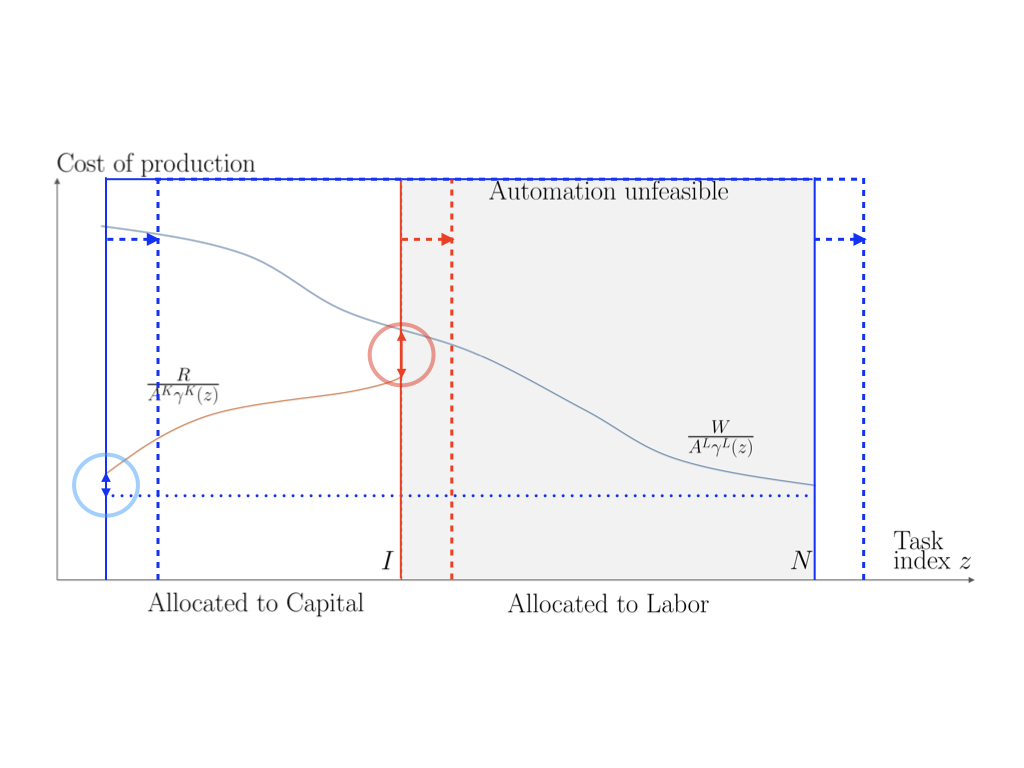
\includegraphics[height=7.5cm,width=\textwidth]{figure1f.png}
\\ Efficiencies at marginal tasks: equilibrium assumptions
\end{figure} 
\end{center}
\newpage

\begin{frame}{Equilibrium assumptions revisited}
\begin{itemize}
\item We assumed that:
\[
\color{red} \frac{A^{L}\gamma^{L}(I)}{A^{K}\gamma^{K}(I)} < \color{black} \frac{W}{R} \color{blue} < \frac{A^{L}\gamma^{L}(N)}{A^{K}\gamma^{K}(N-1)} \color{black} \tag{A1}
\]
\item This is equivalent to assuming \textbf{intermediate values of} $K/L$:
\[
\frac{K}{L} \in (\underline{\kappa}, \overline{\kappa}) \tag{A2} \label{eqA2}
\]
with:
\[
\underline{\kappa} \equiv \frac{I-N+1}{N-I}\frac{\gamma^{L}(I)}{\gamma^{K}(I)} \text{ and } \overline{\kappa} \equiv \frac{I-N+1}{N-I}\frac{\gamma^{L}(N)}{\gamma^{K}(N-1)}
\]
\end{itemize}
\end{frame}

\begin{frame}{Equilibrium assumptions revisited}
\begin{itemize}
\item We had that:
\[
R = \frac{Y}{K}[I-N+1] \text{ and }  W = \frac{Y}{L}[N-I] \tag{5}
\]
\item Combining both equations gives:
\[
\frac{W}{R} = \frac{K}{L} \frac{N-I}{I-N+1}
\]
\item Defining:
\[
\underline{\kappa} \equiv \frac{I-N+1}{N-I}\frac{\gamma^{L}(I)}{\gamma^{K}(I)} \text{ and } \overline{\kappa} \equiv \frac{I-N+1}{N-I}\frac{\gamma^{L}(N)}{\gamma^{K}(N-1)}
\]
then assumption (A2) is equivalent to assumption (A1).
\end{itemize}
\end{frame}

\section{8.4 Technology and Labor Demand}

\begin{frame}{Technological change and labor demand}
\begin{itemize}
\item Types of technological change were (excluding labor augmenting technological change): \medskip
\begin{enumerate}
\item \textbf{Automation (at the extensive margin)}: \\
Automation possibility frontier $I \uparrow $ \medskip
\item \textbf{Deepening of automation (at the intensive margin)}: \\
$\uparrow$ in $\color{cyan} A^{K}$ or $\color{orange} \gamma^{k}(z)$ for all $z < I$ \medskip
\item \textbf{Creation of new labor-intensive tasks}: \\
$N \uparrow $ which increases the bounds of the unit interval of tasks ranked by labor's comparative advantage \smallskip
\end{enumerate}
\item Different types of technological change have different effects on labor demand and the labor share.
\end{itemize}
\end{frame}

\subsection{8.4.1 Automation}

\begin{frame}{8.4 Technology and labor demand}
\begin{itemize}
\item[\textcolor{red}{8.4.1}] \textcolor{red}{Automation} \medskip
\item[\textcolor{gray}{8.4.2}] \textcolor{gray}{Deepening of automation} \medskip
\item[\textcolor{gray}{8.4.3}] \textcolor{gray}{Creation of new labor-intensive tasks} \medskip
\item[\textcolor{gray}{8.4.4}] \textcolor{gray}{A false dichotomy}
\end{itemize}
\end{frame}

\newpage
\begin{center}
\begin{figure}
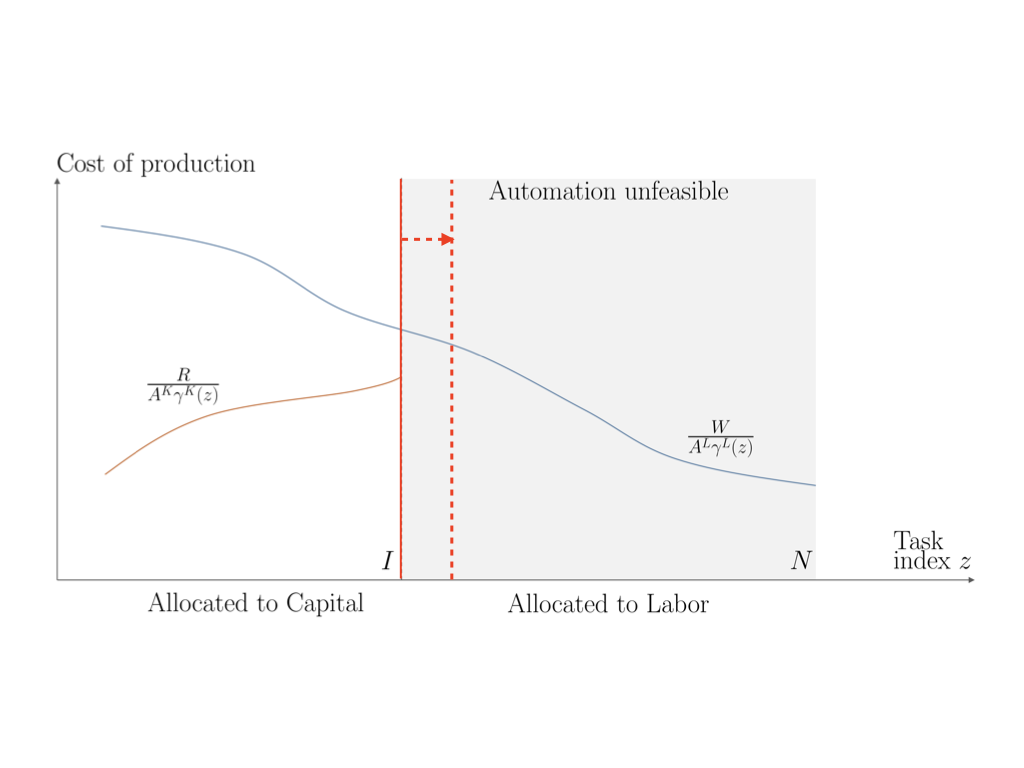
\includegraphics[height=7.5cm,width=\textwidth]{figure2a.png}
\\ 1. \textbf{Automation (at the extensive margin)}: \\
$\rightarrow$ Displacement effect that $ \downarrow$ labor demand
\end{figure} 
\end{center}
\newpage

\begin{frame}{Automation in history}
\begin{itemize}
\item Tasks and automation are at the center of technological change throughout the last 200 years. \medskip
\item Machines and computers have substituted for human labor: \medskip
\begin{itemize}
\item Horse-powered threshing machines replaced manual labor \medskip
\item Machine-tools replaced labor-intensive artisan techniques \medskip
\item Industrial robots automated assembly lines \medskip
\item Software automated tasks by office clerks
\end{itemize}
\end{itemize}
\end{frame}

\newpage
\begin{center}
\begin{figure}
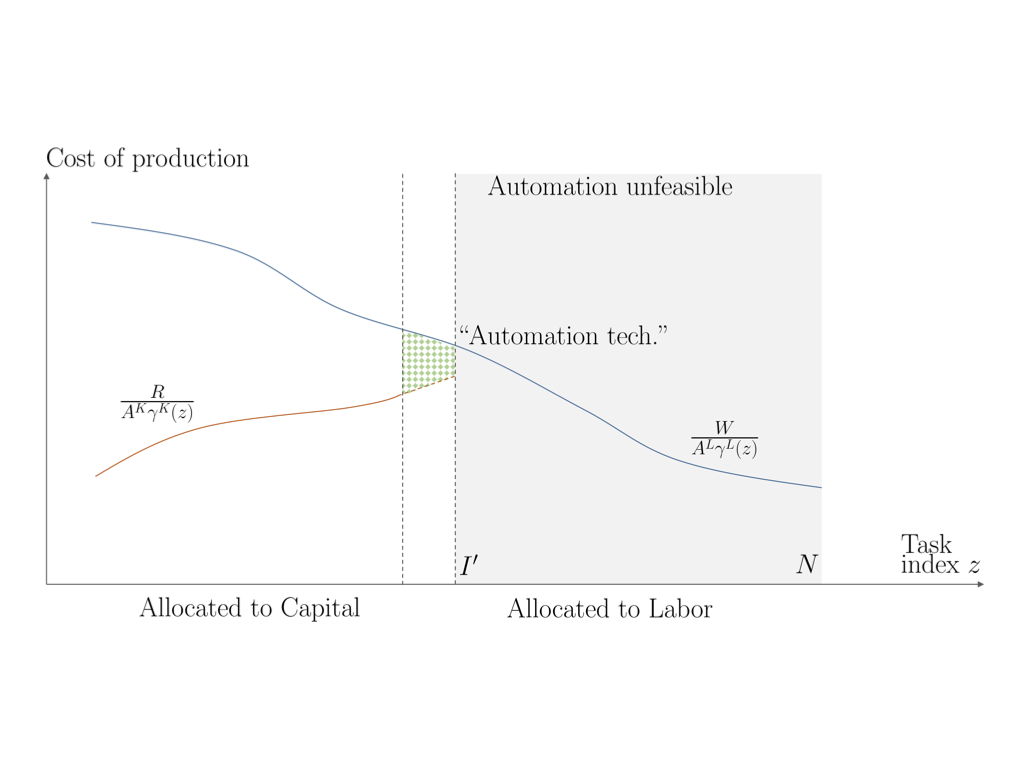
\includegraphics[height=7.5cm,width=\textwidth]{figure1d.png}
\\ 1. \textbf{Automation (at the extensive margin)}: \\
$\rightarrow$ Productivity effect that $ \uparrow$ labor demand
\end{figure} 
\end{center}
\newpage

\begin{frame}{The ambiguous impact of automation on labor demand}
\begin{itemize}
\item We had that:
\[
R = \frac{Y}{K}[I-N+1] \text{ and }  W = \frac{Y}{L}[N-I] \tag{5}
\]
\item Differentiating $\ln(W)$ wrt $I$ gives:
\[
\frac{d\ln(W)}{dI}=\underbrace{\frac{d\ln(N-I)}{dI}}_{\text{Displacement effect}<0} + \underbrace{\frac{d\ln(Y/L)}{dI}}_{\text{Productivity effect}>0} \tag{7} \label{eq7}
\]
\item The impact on labor demand is ambiguous because a negative displacement effect is counteracted by a positive productivity effect.
\end{itemize}
\end{frame}

\begin{frame}{The ambiguous impact of automation on labor demand}
\begin{itemize}
\item Using equations (3)-(5), the productivity effect is given by:
\[
\frac{d\ln(Y/L)}{dI} = \ln \left( \frac{W}{A^{L}\gamma^{L}(I)} \right) - \ln \left( \frac{R}{A^{K}\gamma^{K}(I)} \right) > 0
\]
\item Substituting into equation (7) gives \underline{equation (8)}:
\[
\frac{d\ln(W)}{dI}=\underbrace{-\frac{1}{N-I}}_{\text{Displacement effect}<0} + \underbrace{\ln \left(\frac{W}{A^{L}\gamma^{L}(I)} \right) - \ln \left(\frac{R}{A^{K}\gamma^{K}(I)} \right)}_{\text{Productivity effect}>0} \label{eq8}
\]
\item Displacement effect will dominate the productivity effect if:
\[
\frac{W}{A^{L}\gamma^{L}(I)} \approx \frac{R}{A^{K}\gamma^{K}(I)}
\]
\end{itemize}
\end{frame}

\newpage
\begin{center}
\begin{figure}
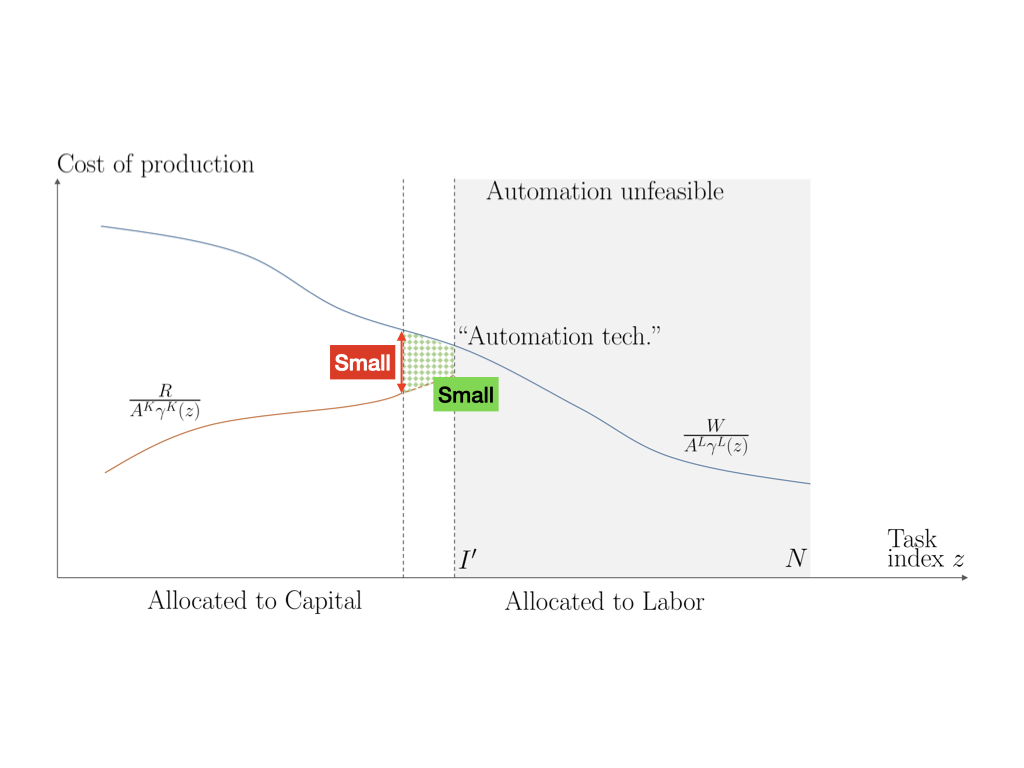
\includegraphics[height=7cm,width=\textwidth]{figure1h.png}
\\ \textbf{Automation when new technologies are ``so-so''}: \\
Displacement effect dominates productivity effect such that labor demand $ \downarrow$
\end{figure} 
\end{center}
\newpage

\begin{frame}{Capital accumulation in the long-run}
\begin{itemize}
\item We had that:
\[
R = \frac{Y}{K}[I-N+1] \text{ and }  W = \frac{Y}{L}[N-I] \tag{5}
\]
\item An increase in $I$ (and $Y$) increases $R$ in the short-run. \medskip
\item This increase in $R$ leads to an increase in $K$ in the long-run (assuming that $R$ is constant in the long-run). \medskip
\item Through q-complementarity, capital accumulation results in an increase in labor demand in the long-run that further counteracts the negative displacement effect.
\end{itemize}
\end{frame}

\begin{frame}{Automation reduces the labor share}
\begin{itemize}
\item We had that:
\[
s_{L} = \frac{WL}{Y} = N-I  = 1 - s_{K} \tag{6}
\]
\item Differentiating $s_{L}$ wrt $I$ gives:
\[
\frac{ds_{L}}{dI} = -1 < 0 \tag{9} \label{eq9}
\]
\item Automation always increases productivity more than the wage:
\[
\frac{d\ln(W)}{dI} - \underbrace{\frac{d\ln(Y/L)}{dI}}_{\text{Productivity effect}>0} =\underbrace{-\frac{1}{N-I}}_{\text{Displacement effect}<0} <0 \tag{7}
\]
\end{itemize}
\end{frame}

\begin{frame}{Automation, labor demand and the labor share}
\begin{itemize}
\item Automation has an ambiguous effect on labor demand because of: \medskip
\begin{enumerate}
\item a negative displacement \medskip
\item a positive productivity effect. \medskip
\end{enumerate}
\item Labor demand decreases when new technologies result in ``so-so automation''. \medskip
\item Automation always reduces the labor share because it increases productivity more than the wage. 
\end{itemize}
\end{frame}

\subsection{8.4.2 Deepening of automation}

\begin{frame}{8.4 Technology and labor demand}
\begin{itemize}
\item[\textcolor{gray}{8.4.1}] \textcolor{gray}{Automation} \medskip
\item[\textcolor{red}{8.4.2}] \textcolor{red}{Deepening of automation} \medskip
\item[\textcolor{gray}{8.4.3}] \textcolor{gray}{Creation of new labor-intensive tasks} \medskip
\item[\textcolor{gray}{8.4.4}] \textcolor{gray}{A false dichotomy}
\end{itemize}
\end{frame}

\newpage
\begin{center}
\begin{figure}
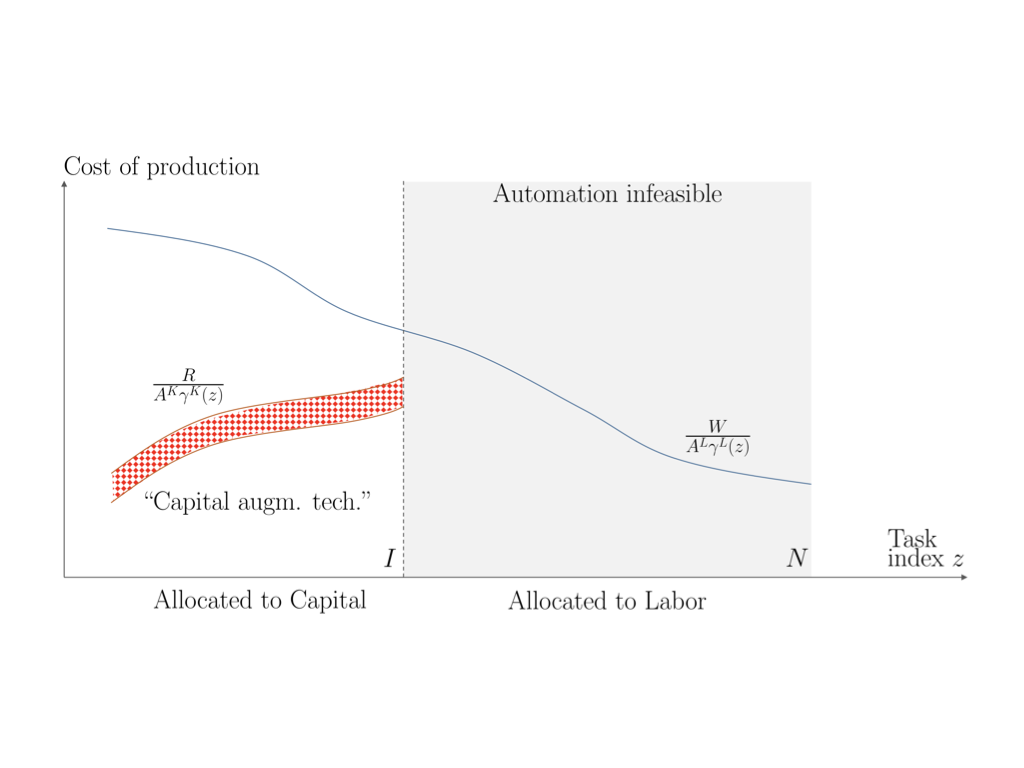
\includegraphics[height=7.5cm,width=\textwidth]{figure1b.png}
\\ 2. \textbf{Deepening of automation (at the intensive margin)}: \\
$ \rightarrow$ Capital deepening that $ \uparrow$ labor demand
\end{figure} 
\end{center}
\newpage

\begin{frame}{Deepening of automation increases labor demand}
\begin{itemize}
\item We had that:
\[
Y = \color{orange} \Pi(I,N) \color{black} \left[ \frac{\color{cyan}A^{K} \color{black}K}{\color{orange}I-N+1} \color{black}\right]^{\color{orange} I-N+1} \color{black} \left[ \frac{\color{cyan}A^{L} \color{black}L}{\color{orange}N-I} \color{black} \right]^{\color{orange} N-I} \tag{3}
\]
\item Assuming $ \color{cyan} A^{K} \color{black} \uparrow$, we get that labor demand increases:
\[
d \ln(W) = d \ln(Y/L) = [I-N+1] d \ln(\color{cyan}A^{K} \color{black} ) > 0
\] 
because of q-complementarity. \medskip
\item There is no impact on the labor share because wages and productivity increase proportionately.
\end{itemize}
\end{frame}

\subsection{8.4.3 New tasks and the comparative advantage of labor}

\begin{frame}{8.4 Technology and labor demand}
\begin{itemize}
\item[\textcolor{gray}{8.4.1}] \textcolor{gray}{Automation} \medskip
\item[\textcolor{gray}{8.4.2}] \textcolor{gray}{Deepening of automation} \medskip
\item[\textcolor{red}{8.4.3}] \textcolor{red}{Creation of new labor-intensive tasks} \medskip
\item[\textcolor{gray}{8.4.4}] \textcolor{gray}{A false dichotomy}
\end{itemize}
\end{frame}

\newpage
\begin{center}
\begin{figure}
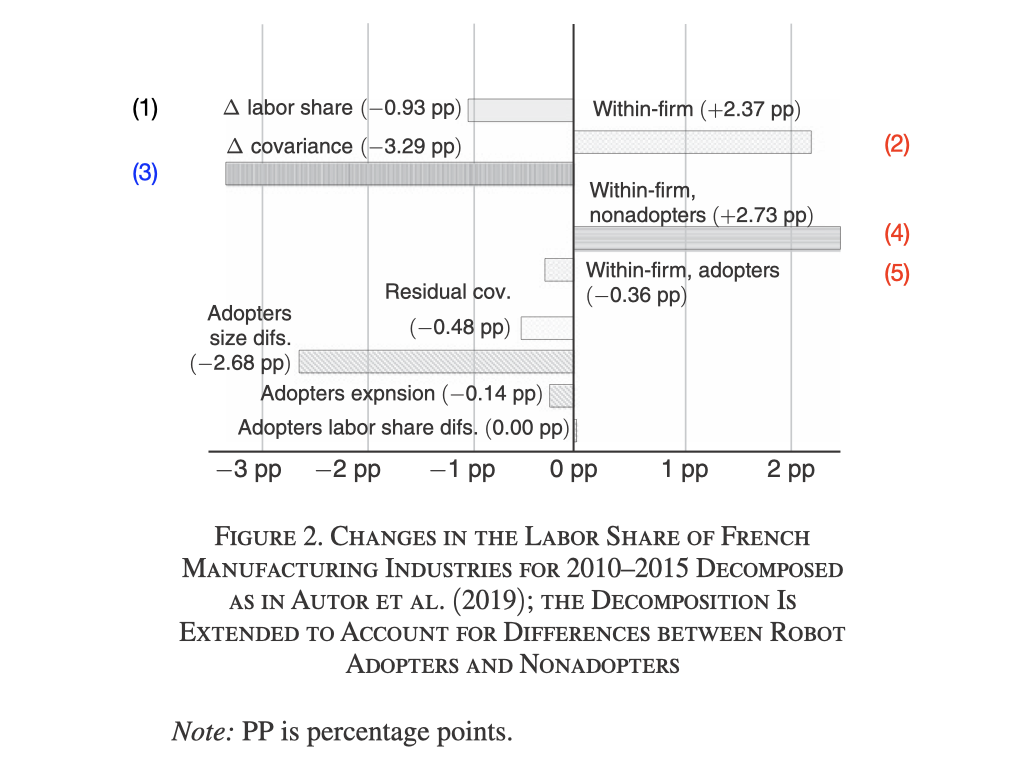
\includegraphics[height=7.5cm,width=\textwidth]{figure2b.png}
\\ 3. \textbf{Creation of new labor-intensive tasks}:\\
$ \rightarrow$ Reinstatement and productivity effect that $ \uparrow $ labor demand
\end{figure} 
\end{center}
\newpage

\begin{frame}{New labor-intensive tasks increase labor demand}
\begin{itemize}
\item We had that:
\[
R = \frac{Y}{K}[I-N+1] \text{ and }  W = \frac{Y}{L}[N-I] \tag{5}
\]
\item Differentiating $\ln(W)$ wrt $N$ gives:
\[
\frac{d\ln(W)}{dN}=\frac{1}{N-I} + \frac{d\ln(Y/L)}{dN}
\] 
\item Differentiating $\ln(Y/L)$ wrt $N$ gives \underline{equation (10)}:
\[
\frac{d\ln(W)}{dN}=\underbrace{\frac{1}{N-I}}_{\text{Reinstatement effect}>0} +   \underbrace{\ln \left( \frac{R}{A^{K}\gamma^{K}(N-1)} / \frac{W}{A^{L}\gamma^{L}(N)} \right) }_{\text{Productivity effect}>0} \label{eq10}
\]
\end{itemize}
\end{frame}

\begin{frame}{New labor-intensive tasks increase the labor share}
\begin{itemize}
\item We had that:
\[
s_{L} = \frac{WL}{Y} = N-I  = 1 - s_{K} \tag{6}
\]
\item Differentiating $s_{L}$ wrt $N$ gives:
\[
\frac{ds_{L}}{dN} = 1 > 0
\]
\item New tasks always increase the wage more than productivity:
\[
\frac{d\ln(W)}{dN} - \underbrace{\frac{d\ln(Y/L)}{dN}}_{\text{Productivity effect}>0} =\underbrace{\frac{1}{N-I}}_{\text{Reinstatement effect}>0} >0
\]
\end{itemize}
\end{frame}

\begin{frame}{Automation, new tasks, and the labor share}
\begin{itemize}
\item Because $s_{L}=N-I$ we have that:
\[
ds_{L}=dN-dI
\]
\item Automation decreases the labor share (despite productivity effects) whereas the creation of new labor-intensive tasks increases the labor share. \medskip
\item A constant labor share suggests that both forces balance each other out, a falling labor share suggests that automation is more important than the creation of new labor intensive tasks.
\item This could also explain why the labor share was constant before 2000 (but not afterward).
\end{itemize}
\end{frame}

\begin{frame}{Balanced growth and directed technological change}
\begin{itemize}
\item A full model endogenizes capital accumulation and the direction of research toward automation, $dI$, and the creation of new tasks, $dN$. \medskip
\item Acemoglu \& Restrepo [18] show that there exists a stable balanced growth path in which $dI=dN$. \medskip 
\item In steady-state, real wages grow because automation and new task creation happen simultaneously but are labor-augmenting on net because labor becomes more productive in new tasks. \medskip
\item What these new labor task exactly are remains ``dark matter'' (i.e. forceful but unknown).
\end{itemize}
\end{frame}

\subsection{8.4.4 A false dichotomy}

\begin{frame}{8.4 Technology and labor demand}
\begin{itemize}
\item[\textcolor{gray}{8.4.1}] \textcolor{gray}{Automation} \medskip
\item[\textcolor{gray}{8.4.2}] \textcolor{gray}{Deepening of automation} \medskip
\item[\textcolor{gray}{8.4.3}] \textcolor{gray}{Creation of new labor-intensive tasks} \medskip
\item[\textcolor{red}{8.4.4}] \textcolor{red}{A false dichotomy}
\end{itemize}
\end{frame}

\begin{frame}{A false dichotomy}
\begin{itemize}
\item The public debate is often centered around the false dichotomy between disastrous and totally benign effects of automation. \medskip
\item A task-based framework is more nuanced. \medskip
\item It underscores that automation could reduce wages, employment, and the labor share. \medskip
\item There is a lot of theoretical and empirical research on the way that is digging deeper into these nuances.
\end{itemize}
\end{frame}

\section{8.5 Flies in the Ointment}

\begin{frame}{Flies in the ointment}
\begin{itemize}
\item In the baseline model, the reallocation of capital and labor across tasks due to $dI$ and $dN$ is frictionless. \medskip 
\item The baseline model underplays the importance of adjustment costs and inefficiencies. \medskip
\item In this section, we focus on the impact of $dI$ on $dY$ assuming several inefficiencies. \medskip
\item We could also look at the impact of $dN$ assuming the same or other inefficiences.
\end{itemize}
\end{frame}

\begin{frame}{Models of automation with inefficiencies}
\begin{itemize}
\item We adjust the baseline model of automation by adding either of three inefficiencies: \medskip
\begin{enumerate}
\item Technology-skill mismatch \medskip
\item Biased taxes that subsidize capital relative to labor \medskip
\item Labor market imperfections that result in wage rents \medskip
\end{enumerate}
\item Inefficiencies in these models result in the misallocation of factors in equilibrium. In particular, demand for capital relative to labor is too high (near $I$). \medskip
\item These inefficiencies mitigate the positive impact of $dI$ on $dY$ and their rise could explain missing productivity growth.
\end{itemize}
\end{frame}

\subsection{8.5.1 Mismatch of technologies and skills}

\begin{frame}{8.5 Flies in the Ointment}
\begin{itemize}
\item[\textcolor{red}{8.5.1}] \textcolor{red}{Mismatch of technologies and skills} \bigskip
\item[\textcolor{gray}{8.5.2}] \textcolor{gray}{Biased taxes that subsidize capital relative to labor} \bigskip
\item[\textcolor{gray}{8.5.3}] \textcolor{gray}{Labor market imperfections with wage rents}
\end{itemize}
\end{frame}

\begin{frame}{A model with technology-skill mismatch}
Assume that:
\begin{enumerate}
\item Low-skill workers supply $L$ and high-skill workers supply $H$. \medskip
\item Low-skill workers can only perform tasks below a threshold $S \in (I,N)$ with lower $S$ capturing higher technology-skill mismatch (high-skilled workers can still do all tasks). \medskip
\item Productivity of low-skill and high-skill workers is given by $A^{L} \gamma^{L}(z)$ (differential advantages are possible, but the more restrictive assumption here is 2). \medskip
\item Low-skill workers earn a wage $W^{L}$ and high-skill workers earn a wage $W^{H}>W^{L}$ in equilibrium.
\end{enumerate}
\end{frame}

\begin{frame}{Technology-skill mismatch and wage inequality}
\begin{itemize}
\item Following the same steps as in the baseline model gives:
\[
R=\frac{Y}{K}[I-N+1] \text{ ; } W^{H}=\frac{Y}{H}[N-S] \text{ ; } W^{L}=\frac{Y}{L}[S-I]
\]
\item Differentiating $\ln(W^{H}/W^{L})$ wrt $I$ gives:
\[
\frac{d\ln(W^{H}/W^{L})}{dI} = \frac{1}{S-I} > 0
\]
\item This increase is larger if $S$ is lower, i.e. if technology-skill mismatch is higher, because displaced low-skilled workers will be squeezed into an even smaller set of tasks.
\end{itemize}
\end{frame}

\begin{frame}{Technology-skill mismatch and productivity}
\begin{itemize}
\item Following the same steps as in the baseline model:
\[
\frac{d\ln(Y/L)}{dI} = \ln \left(\frac{W^{L}}{A^{L}\gamma^{L}(I)} \right) - \ln \left(\frac{R}{A^{K}\gamma^{K}(I)} \right) > 0
\]
\item We also have that:
\[
\frac{W^{L}}{R} = \frac{S-I}{I-N+1} \frac{K}{L}
\]
\item A worse mismatch (lower $S$) and therefore lower $W^{L}/R$ reduces the productivity gains from automation.
\end{itemize}
\end{frame}

\begin{frame}{Policy implications}
\begin{itemize}
\item Technology-skill mismatch (i.e. $S<N$) results in a misallocation because unskilled workers do too few tasks given their limited task mobility. \medskip
\item If $dI$ automates the task of workers with limited mobility, the productivity gains from automation are lower. \medskip
\item Policies that increase $S$ are education, training, and active labor market policies targeted to displaced workers. \medskip
\item E.g. Productivity growth from automation in the early 20th-century was aided by the ``high-school movement''.
\end{itemize}
\end{frame}

\subsection{8.5.2 Biased taxes that subsidize capital relative to labor}

\begin{frame}{8.5 Flies in the Ointment}
\begin{itemize}
\item[\textcolor{gray}{8.5.1}] \textcolor{gray}{Mismatch of technologies and skills} \bigskip
\item[\textcolor{red}{8.5.2}] \textcolor{red}{Biased taxes that subsidize capital relative to labor} \bigskip
\item[\textcolor{gray}{8.5.3}] \textcolor{gray}{Labor market imperfections with wage rents}
\end{itemize}
\end{frame}

\begin{frame}{A model with taxes that subsidize capital relative to labor}
\begin{itemize}
\item Assume that: \medskip
\begin{enumerate}
\item Capital $K$ is no longer fixed but produced as an intermediate good at fixed cost $R$, using the final good as an input. \medskip
\item The use of capital $K$ in final good production receives a marginal subsidy of $\tau>0$ such that the rental rate is $[1-\tau]R$. \medskip
\item Subsidy $\tau$ can be a tax credit for investments or income taxes that subsidizes capital (relative to labor). \medskip
\end{enumerate}
\item There will be too much capital produced by the intermediate sector (which requires resources), and this will mitigate the impact of $dI$ on $d(GDP \equiv Y-RK)$. 
\end{itemize}
\end{frame}

\begin{frame}{Capital subsidies, automation and productivity}
\begin{itemize}
\item Define $GDP$ as value-added output:
\[
GDP \equiv Y - RK
\]
with $Y$ the value of final goods production and $RK$ the cost of producing capital. \medskip
\item The impact of automation on $GDP$ is then given by:
\[
\frac{dGDP}{dI} = \frac{dY}{dI} |_{K} + [1-\tau]R \frac{dK}{dI} - R\frac{dK}{dI}
\]
\item The first term gives the impact of $dI$ on $Y$ for given $K$ as in the baseline model, and the last two terms account for the impact of $dI$ on capital accumulation.
\end{itemize}
\end{frame}

\begin{frame}{Capital subsidies, automation and productivity}
\begin{itemize}
\item The change in value added $GDP$ due to automation was:
\[
\frac{dGDP}{dI} = \frac{dY}{dI} |_{K} + [1-\tau]R \frac{dK}{dI} - R\frac{dK}{dI}
\]
\item The first term in the right-hand side is a productivity effect as in the baseline model:
\begin{align*}
\frac{dGDP}{dI} & = \underbrace{\left[ \ln \left( \frac{W}{A^{L}\gamma^{L}(I)} \right) - \ln \left( \frac{[1- \tau ]R}{A^{K}\gamma^{K}(I)} \right) \right]Y}_{\text{Productivity effect }>0} \\
& \underbrace{ -\tau R \frac{dK}{dI}}_{\text{Capital subsidy effect } <0}
\end{align*}
where the last term is negative given that $dK/dI >0$.
\end{itemize}
\end{frame}

\begin{frame}{Policy implications}
\begin{itemize}
\item Automation increases productivity, but taxes that subsidize capital relative to labor could lower this productivity gain. \medskip
\item The reason is that tax codes that subsidize capital relative to labor result in capital accumulation that could be costly. \medskip
\item Current tax codes heavily favor capital income and capital investments over payroll taxes. \medskip
\item A more titled playing field leads to a slowdown in productivity growth.
\end{itemize}
\end{frame}

\subsection{8.5.3 Labor market imperfections with wage rents}

\begin{frame}{8.5 Flies in the Ointment}
\begin{itemize}
\item[\textcolor{gray}{8.5.1}] \textcolor{gray}{Mismatch of technologies and skills} \bigskip
\item[\textcolor{gray}{8.5.2}] \textcolor{gray}{Biased taxes that subsidize capital relative to labor} \bigskip
\item[\textcolor{red}{8.5.3}] \textcolor{red}{Labor market imperfections with wage rents}
\end{itemize}
\end{frame}

\begin{frame}{A model with wage rents}
\begin{itemize}
\item Assume that $L_{A}$ workers in tasks $(I,J)$ with $J \in (I,N)$ earn a marginal wage rent $\omega >0$, such that their wage is $[1+ \omega]W$ compared to $L-L_{A}$ workers in tasks $[J,N]$ who earn $W$. \medskip
\item Rents $\omega>0$ could capture unionized jobs or sectors, efficiency wages, or result from other labor market frictions (but we have to be on the labor demand curve). \medskip
\item Wage rents imply that $L_{A}$ will be too low relative to $L-L_{A}$ from a social point of view. \medskip
\item Automation of tasks done by $L_{A}$ workers will worsen this misallocation. 
\end{itemize}
\end{frame}

\begin{frame}{Wage rents and the misallocation of labor}
\begin{itemize}
\item Following similar steps as in the baseline model, the demand for $L_{A}$ is given by:
\[
L_{A} = \frac{Y}{[1+\omega ]W}[J-I]
\]
\item Demand for $L-L_{A}$ is given by:
\[
L-L_{A} = \frac{Y}{W}[N-J]
\]
\item Relative demand for $L_{A}$ is given by:
\[
\frac{L_{A}}{L-L_{A}} = \frac{1}{1+ \omega } \frac{J-I}{N-J}
\]
which is decreasing in $\omega$ and $I$.
\end{itemize}
\end{frame}

\begin{frame}{Wage rents, automation and productivity}
\begin{itemize}
\item The change in $Y$ due to automation is given by:
\[
\frac{dY}{dI} = \frac{dY}{dI} |_{L_{a}} + [1+ \omega]W\frac{dL_{A}}{dI} +W\frac{d[L-L_{A}]}{dI}
\]
\item The first term in the right-hand side is a productivity effect as in the baseline model:
\begin{align*}
\frac{dY}{dI} & = \underbrace{\left[ \ln \left( \frac{[1+ \omega]W}{A^{L}\gamma^{L}(I)} \right) - \ln \left( \frac{R}{A^{K}\gamma^{K}(I)} \right) \right]Y}_{\text{Productivity effect }>0} \\
& \underbrace{ +\omega W \frac{dL_{A}}{dI}}_{\text{Excessive displacement of labor effect } <0}
\end{align*}
where the last term is negative given that $dL_{A}/dI <0$.
\end{itemize}
\end{frame}

\begin{frame}{Policy implications}
\begin{itemize}
\item Automation increases output, but wage rents in automated jobs lower this productivity gain. \medskip
\item The reason is that wage rents result in too few workers in automatable jobs where labor productivity is higher and too many workers in other jobs where labor productivity is lower. \medskip
\item Automation makes this misallocation worse by displacing workers from high productivity to low productivity jobs. \medskip
\item Increasing wage rents in automatable jobs create a slowdown in productivity growth.
\end{itemize}
\end{frame}

\begin{frame}{Automation, new tasks and missing productivity growth}
A deep puzzle is missing productivity growth. Task-based frameworks give several possible explanations: \medskip
\begin{enumerate}
\item \underline{$dI, dN, d[A^{K}\gamma^{K}],d[A^{L}\gamma^{L}] \downarrow$}: Technological progress is $\downarrow$ \medskip
\item \underline{$dI \uparrow$ and $dN \downarrow$} and the productivity gains from $dI$ are less than from $dN$ (e.g. so-so automation). \medskip
\item \underline{$dN \uparrow$ and $dI \downarrow$} and the productivity gains from $dN$ are less than from $dI$ (e.g. new ``green jobs''). \medskip
\item Technology-skill mismatch $ \uparrow$ \medskip
\item Subsidization of capital relative to labor $ \uparrow$ \medskip
\item Wage rents for workers in automatable jobs $ \uparrow$
\end{enumerate}
\end{frame}

\section{8.6 Conclusions}

\begin{frame}{Conclusions}
\begin{itemize}
\item Discussions about automation and the future of work lack a conceptual framework. \medskip
\item A task-based framework provides such a conceptual framework. \medskip
\item It is a rich environment that includes factor-augmenting technologies, automation at the extensive and intensive margin, and the creation of new labor-intensive tasks. \medskip 
\item It (better) explains why wages of some workers have declined, and why the labor share has been falling. \medskip
\item It illustrates how several inefficiencies can be a drag on productivity growth.
\end{itemize}
\end{frame}

\end{document}
